\documentclass[1p]{elsarticle_modified}
%\bibliographystyle{elsarticle-num}

%\usepackage[colorlinks]{hyperref}
%\usepackage{abbrmath_seonhwa} %\Abb, \Ascr, \Acal ,\Abf, \Afrak
\usepackage{amsfonts}
\usepackage{amssymb}
\usepackage{amsmath}
\usepackage{amsthm}
\usepackage{scalefnt}
\usepackage{amsbsy}
\usepackage{kotex}
\usepackage{caption}
\usepackage{subfig}
\usepackage{color}
\usepackage{graphicx}
\usepackage{xcolor} %% white, black, red, green, blue, cyan, magenta, yellow
\usepackage{float}
\usepackage{setspace}
\usepackage{hyperref}

\usepackage{tikz}
\usetikzlibrary{arrows}

\usepackage{multirow}
\usepackage{array} % fixed length table
\usepackage{hhline}

%%%%%%%%%%%%%%%%%%%%%
\makeatletter
\renewcommand*\env@matrix[1][\arraystretch]{%
	\edef\arraystretch{#1}%
	\hskip -\arraycolsep
	\let\@ifnextchar\new@ifnextchar
	\array{*\c@MaxMatrixCols c}}
\makeatother %https://tex.stackexchange.com/questions/14071/how-can-i-increase-the-line-spacing-in-a-matrix
%%%%%%%%%%%%%%%

\usepackage[normalem]{ulem}

\newcommand{\msout}[1]{\ifmmode\text{\sout{\ensuremath{#1}}}\else\sout{#1}\fi}
%SOURCE: \msout is \stkout macro in https://tex.stackexchange.com/questions/20609/strikeout-in-math-mode

\newcommand{\cancel}[1]{
	\ifmmode
	{\color{red}\msout{#1}}
	\else
	{\color{red}\sout{#1}}
	\fi
}

\newcommand{\add}[1]{
	{\color{blue}\uwave{#1}}
}

\newcommand{\replace}[2]{
	\ifmmode
	{\color{red}\msout{#1}}{\color{blue}\uwave{#2}}
	\else
	{\color{red}\sout{#1}}{\color{blue}\uwave{#2}}
	\fi
}

\newcommand{\Sol}{\mathcal{S}} %segment
\newcommand{\D}{D} %diagram
\newcommand{\A}{\mathcal{A}} %arc


%%%%%%%%%%%%%%%%%%%%%%%%%%%%%5 test

\def\sl{\operatorname{\textup{SL}}(2,\Cbb)}
\def\psl{\operatorname{\textup{PSL}}(2,\Cbb)}
\def\quan{\mkern 1mu \triangleright \mkern 1mu}

\theoremstyle{definition}
\newtheorem{thm}{Theorem}[section]
\newtheorem{prop}[thm]{Proposition}
\newtheorem{lem}[thm]{Lemma}
\newtheorem{ques}[thm]{Question}
\newtheorem{cor}[thm]{Corollary}
\newtheorem{defn}[thm]{Definition}
\newtheorem{exam}[thm]{Example}
\newtheorem{rmk}[thm]{Remark}
\newtheorem{alg}[thm]{Algorithm}

\newcommand{\I}{\sqrt{-1}}
\begin{document}

%\begin{frontmatter}
%
%\title{Boundary parabolic representations of knots up to 8 crossings}
%
%%% Group authors per affiliation:
%\author{Yunhi Cho} 
%\address{Department of Mathematics, University of Seoul, Seoul, Korea}
%\ead{yhcho@uos.ac.kr}
%
%
%\author{Seonhwa Kim} %\fnref{s_kim}}
%\address{Center for Geometry and Physics, Institute for Basic Science, Pohang, 37673, Korea}
%\ead{ryeona17@ibs.re.kr}
%
%\author{Hyuk Kim}
%\address{Department of Mathematical Sciences, Seoul National University, Seoul 08826, Korea}
%\ead{hyukkim@snu.ac.kr}
%
%\author{Seokbeom Yoon}
%\address{Department of Mathematical Sciences, Seoul National University, Seoul, 08826,  Korea}
%\ead{sbyoon15@snu.ac.kr}
%
%\begin{abstract}
%We find all boundary parabolic representation of knots up to 8 crossings.
%
%\end{abstract}
%\begin{keyword}
%    \MSC[2010] 57M25 
%\end{keyword}
%
%\end{frontmatter}

%\linenumbers
%\tableofcontents
%
\newcommand\colored[1]{\textcolor{white}{\rule[-0.35ex]{0.8em}{1.4ex}}\kern-0.8em\color{red} #1}%
%\newcommand\colored[1]{\textcolor{white}{ #1}\kern-2.17ex	\textcolor{white}{ #1}\kern-1.81ex	\textcolor{white}{ #1}\kern-2.15ex\color{red}#1	}

{\Large $\underline{12a_{0492}~(K12a_{0492})}$}

\setlength{\tabcolsep}{10pt}
\renewcommand{\arraystretch}{1.6}
\vspace{1cm}\begin{tabular}{m{100pt}>{\centering\arraybackslash}m{274pt}}
\multirow{5}{120pt}{
	\centering
	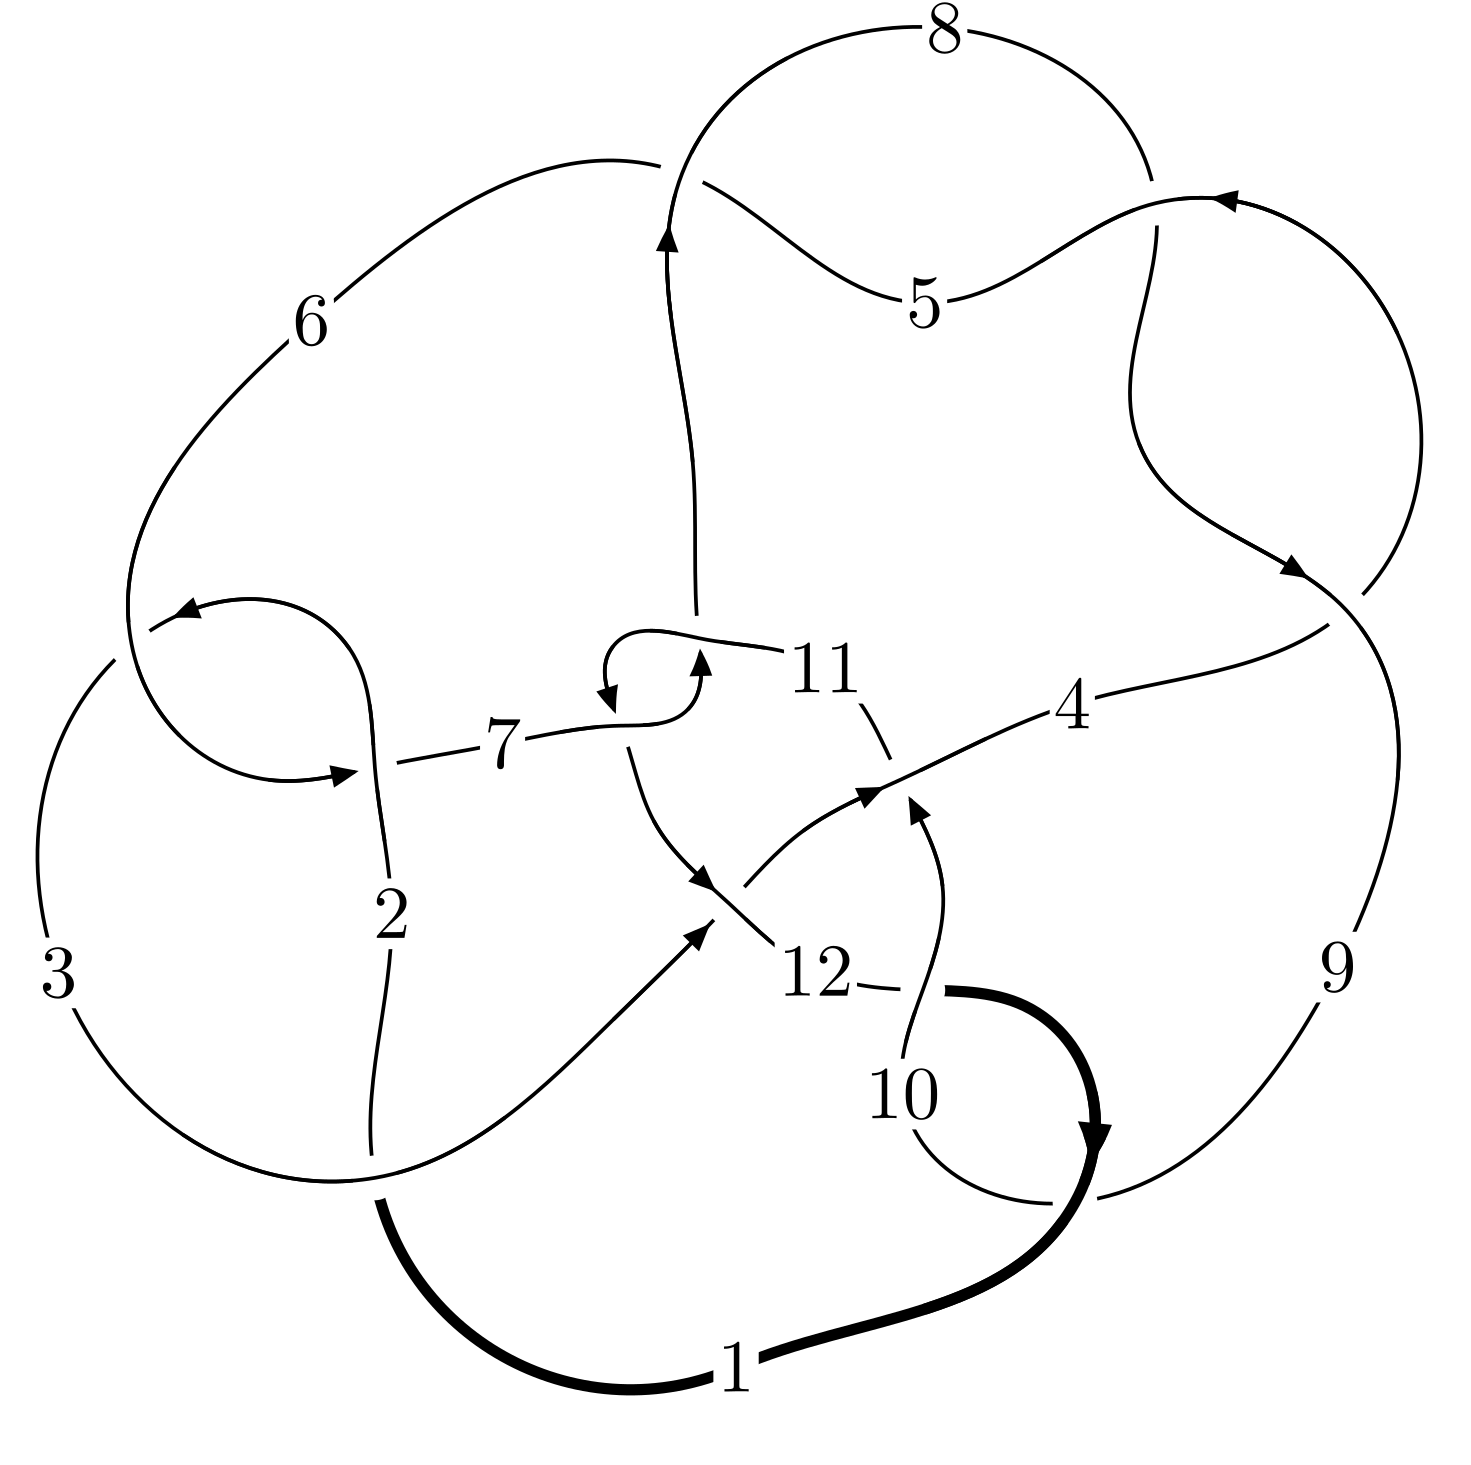
\includegraphics[width=112pt]{../../../GIT/diagram.site/Diagrams/png/1293_12a_0492.png}\\
\ \ \ A knot diagram\footnotemark}&
\allowdisplaybreaks
\textbf{Linearized knot diagam} \\
\cline{2-2}
 &
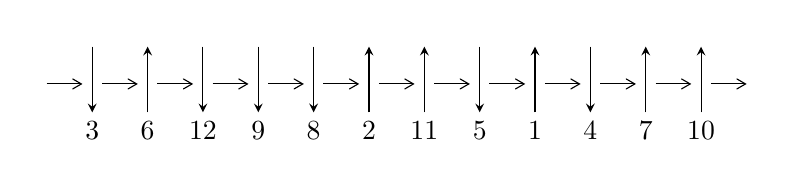
\begin{tikzpicture}[x=20pt, y=17pt]
	% nodes
	\node (C0) at (0, 0) {};
	\node (C1) at (1, 0) {};
	\node (C1U) at (1, +1) {};
	\node (C1D) at (1, -1) {3};

	\node (C2) at (2, 0) {};
	\node (C2U) at (2, +1) {};
	\node (C2D) at (2, -1) {6};

	\node (C3) at (3, 0) {};
	\node (C3U) at (3, +1) {};
	\node (C3D) at (3, -1) {12};

	\node (C4) at (4, 0) {};
	\node (C4U) at (4, +1) {};
	\node (C4D) at (4, -1) {9};

	\node (C5) at (5, 0) {};
	\node (C5U) at (5, +1) {};
	\node (C5D) at (5, -1) {8};

	\node (C6) at (6, 0) {};
	\node (C6U) at (6, +1) {};
	\node (C6D) at (6, -1) {2};

	\node (C7) at (7, 0) {};
	\node (C7U) at (7, +1) {};
	\node (C7D) at (7, -1) {11};

	\node (C8) at (8, 0) {};
	\node (C8U) at (8, +1) {};
	\node (C8D) at (8, -1) {5};

	\node (C9) at (9, 0) {};
	\node (C9U) at (9, +1) {};
	\node (C9D) at (9, -1) {1};

	\node (C10) at (10, 0) {};
	\node (C10U) at (10, +1) {};
	\node (C10D) at (10, -1) {4};

	\node (C11) at (11, 0) {};
	\node (C11U) at (11, +1) {};
	\node (C11D) at (11, -1) {7};

	\node (C12) at (12, 0) {};
	\node (C12U) at (12, +1) {};
	\node (C12D) at (12, -1) {10};
	\node (C13) at (13, 0) {};

	% arrows
	\draw[->,>={angle 60}]
	(C0) edge (C1) (C1) edge (C2) (C2) edge (C3) (C3) edge (C4) (C4) edge (C5) (C5) edge (C6) (C6) edge (C7) (C7) edge (C8) (C8) edge (C9) (C9) edge (C10) (C10) edge (C11) (C11) edge (C12) (C12) edge (C13) ;	\draw[->,>=stealth]
	(C1U) edge (C1D) (C2D) edge (C2U) (C3U) edge (C3D) (C4U) edge (C4D) (C5U) edge (C5D) (C6D) edge (C6U) (C7D) edge (C7U) (C8U) edge (C8D) (C9D) edge (C9U) (C10U) edge (C10D) (C11D) edge (C11U) (C12D) edge (C12U) ;
	\end{tikzpicture} \\
\hhline{~~} \\& 
\textbf{Solving Sequence} \\ \cline{2-2} 
 &
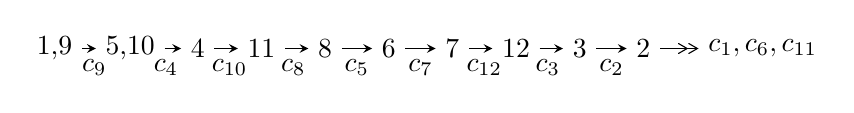
\begin{tikzpicture}[x=23pt, y=7pt]
	% node
	\node (A0) at (-1/8, 0) {1,9};
	\node (A1) at (17/16, 0) {5,10};
	\node (A2) at (17/8, 0) {4};
	\node (A3) at (25/8, 0) {11};
	\node (A4) at (33/8, 0) {8};
	\node (A5) at (41/8, 0) {6};
	\node (A6) at (49/8, 0) {7};
	\node (A7) at (57/8, 0) {12};
	\node (A8) at (65/8, 0) {3};
	\node (A9) at (73/8, 0) {2};
	\node (C1) at (1/2, -1) {$c_{9}$};
	\node (C2) at (13/8, -1) {$c_{4}$};
	\node (C3) at (21/8, -1) {$c_{10}$};
	\node (C4) at (29/8, -1) {$c_{8}$};
	\node (C5) at (37/8, -1) {$c_{5}$};
	\node (C6) at (45/8, -1) {$c_{7}$};
	\node (C7) at (53/8, -1) {$c_{12}$};
	\node (C8) at (61/8, -1) {$c_{3}$};
	\node (C9) at (69/8, -1) {$c_{2}$};
	\node (A10) at (11, 0) {$c_{1},c_{6},c_{11}$};

	% edge
	\draw[->,>=stealth]	
	(A0) edge (A1) (A1) edge (A2) (A2) edge (A3) (A3) edge (A4) (A4) edge (A5) (A5) edge (A6) (A6) edge (A7) (A7) edge (A8) (A8) edge (A9) ;
	\draw[->>,>={angle 60}]	
	(A9) edge (A10);
\end{tikzpicture} \\ 

\end{tabular} \\

\footnotetext{
The image of knot diagram is generated by the software ``\textbf{Draw programme}" developed by Andrew Bartholomew(\url{http://www.layer8.co.uk/maths/draw/index.htm\#Running-draw}), where we modified some parts for our purpose(\url{https://github.com/CATsTAILs/LinksPainter}).
}\phantom \\ \newline 
\centering \textbf{Ideals for irreducible components\footnotemark of $X_{\text{par}}$} 
 
\begin{align*}
I^u_{1}&=\langle 
4.49532\times10^{457} u^{131}+1.34440\times10^{459} u^{130}+\cdots+7.49258\times10^{458} b-7.19414\times10^{459},\\
\phantom{I^u_{1}}&\phantom{= \langle  }1.32939\times10^{460} u^{131}-5.25151\times10^{460} u^{130}+\cdots+5.24480\times10^{459} a-8.37691\times10^{461},\\
\phantom{I^u_{1}}&\phantom{= \langle  }u^{132}-3 u^{131}+\cdots-163 u+7\rangle \\
I^u_{2}&=\langle 
1904483 u^{33}+10211296 u^{32}+\cdots+32131 b-1103768,\\
\phantom{I^u_{2}}&\phantom{= \langle  }142988 u^{33}+2782382 u^{32}+\cdots+32131 a+2978401,\;u^{34}+6 u^{33}+\cdots+6 u+1\rangle \\
\\
\end{align*}
\raggedright * 2 irreducible components of $\dim_{\mathbb{C}}=0$, with total 166 representations.\\
\footnotetext{All coefficients of polynomials are rational numbers. But the coefficients are sometimes approximated in decimal forms when there is not enough margin.}
\newpage
\renewcommand{\arraystretch}{1}
\centering \section*{I. $I^u_{1}= \langle 4.50\times10^{457} u^{131}+1.34\times10^{459} u^{130}+\cdots+7.49\times10^{458} b-7.19\times10^{459},\;1.33\times10^{460} u^{131}-5.25\times10^{460} u^{130}+\cdots+5.24\times10^{459} a-8.38\times10^{461},\;u^{132}-3 u^{131}+\cdots-163 u+7 \rangle$}
\flushleft \textbf{(i) Arc colorings}\\
\begin{tabular}{m{7pt} m{180pt} m{7pt} m{180pt} }
\flushright $a_{1}=$&$\begin{pmatrix}0\\u\end{pmatrix}$ \\
\flushright $a_{9}=$&$\begin{pmatrix}1\\0\end{pmatrix}$ \\
\flushright $a_{5}=$&$\begin{pmatrix}-2.53469 u^{131}+10.0128 u^{130}+\cdots-2944.38 u+159.718\\-0.0599970 u^{131}-1.79431 u^{130}+\cdots-93.1612 u+9.60169\end{pmatrix}$ \\
\flushright $a_{10}=$&$\begin{pmatrix}1\\- u^2\end{pmatrix}$ \\
\flushright $a_{4}=$&$\begin{pmatrix}-2.59468 u^{131}+8.21848 u^{130}+\cdots-3037.54 u+169.320\\-0.0599970 u^{131}-1.79431 u^{130}+\cdots-93.1612 u+9.60169\end{pmatrix}$ \\
\flushright $a_{11}=$&$\begin{pmatrix}-2.43235 u^{131}+4.13228 u^{130}+\cdots-933.324 u+44.4441\\1.61308 u^{131}-3.00750 u^{130}+\cdots+74.0594 u-6.86179\end{pmatrix}$ \\
\flushright $a_{8}=$&$\begin{pmatrix}4.08367 u^{131}-9.26283 u^{130}+\cdots+689.628 u-30.4569\\-2.56390 u^{131}+5.88147 u^{130}+\cdots-255.427 u+15.1075\end{pmatrix}$ \\
\flushright $a_{6}=$&$\begin{pmatrix}-6.51879 u^{131}+19.3840 u^{130}+\cdots-5603.96 u+307.796\\-1.20351 u^{131}+6.16996 u^{130}+\cdots-939.632 u+43.8102\end{pmatrix}$ \\
\flushright $a_{7}=$&$\begin{pmatrix}8.38214 u^{131}-20.0903 u^{130}+\cdots+3504.62 u-174.236\\-0.522846 u^{131}-0.996017 u^{130}+\cdots+146.734 u-3.59969\end{pmatrix}$ \\
\flushright $a_{12}=$&$\begin{pmatrix}- u\\u^3+u\end{pmatrix}$ \\
\flushright $a_{3}=$&$\begin{pmatrix}-3.29886 u^{131}+11.0378 u^{130}+\cdots-3275.81 u+180.206\\0.395435 u^{131}-3.87090 u^{130}+\cdots+24.9734 u+3.66305\end{pmatrix}$ \\
\flushright $a_{2}=$&$\begin{pmatrix}7.10298 u^{131}-19.9316 u^{130}+\cdots+3764.18 u-177.090\\0.709157 u^{131}-1.17970 u^{130}+\cdots-83.6983 u+6.23531\end{pmatrix}$\\&\end{tabular}
\flushleft \textbf{(ii) Obstruction class $= -1$}\\~\\
\flushleft \textbf{(iii) Cusp Shapes $= 1.14347 u^{131}-7.73109 u^{130}+\cdots+1768.78 u-99.4316$}\\~\\
\newpage\renewcommand{\arraystretch}{1}
\flushleft \textbf{(iv) u-Polynomials at the component}\newline \\
\begin{tabular}{m{50pt}|m{274pt}}
Crossings & \hspace{64pt}u-Polynomials at each crossing \\
\hline $$\begin{aligned}c_{1}\end{aligned}$$&$\begin{aligned}
&u^{132}+58 u^{131}+\cdots+174793220 u+8300161
\end{aligned}$\\
\hline $$\begin{aligned}c_{2},c_{6}\end{aligned}$$&$\begin{aligned}
&u^{132}+29 u^{130}+\cdots-9092 u+2881
\end{aligned}$\\
\hline $$\begin{aligned}c_{3}\end{aligned}$$&$\begin{aligned}
&u^{132}-3 u^{131}+\cdots+11521 u+305
\end{aligned}$\\
\hline $$\begin{aligned}c_{4},c_{5},c_{8}\end{aligned}$$&$\begin{aligned}
&u^{132}-3 u^{131}+\cdots-323 u+29
\end{aligned}$\\
\hline $$\begin{aligned}c_{7},c_{11}\end{aligned}$$&$\begin{aligned}
&u^{132}-3 u^{131}+\cdots-1032 u+187
\end{aligned}$\\
\hline $$\begin{aligned}c_{9},c_{12}\end{aligned}$$&$\begin{aligned}
&u^{132}+3 u^{131}+\cdots+163 u+7
\end{aligned}$\\
\hline $$\begin{aligned}c_{10}\end{aligned}$$&$\begin{aligned}
&u^{132}+u^{131}+\cdots+27596 u+6781
\end{aligned}$\\
\hline
\end{tabular}\\~\\
\newpage\renewcommand{\arraystretch}{1}
\flushleft \textbf{(v) Riley Polynomials at the component}\newline \\
\begin{tabular}{m{50pt}|m{274pt}}
Crossings & \hspace{64pt}Riley Polynomials at each crossing \\
\hline $$\begin{aligned}c_{1}\end{aligned}$$&$\begin{aligned}
&y^{132}+50 y^{131}+\cdots+932283187604884 y+68892672625921
\end{aligned}$\\
\hline $$\begin{aligned}c_{2},c_{6}\end{aligned}$$&$\begin{aligned}
&y^{132}+58 y^{131}+\cdots+174793220 y+8300161
\end{aligned}$\\
\hline $$\begin{aligned}c_{3}\end{aligned}$$&$\begin{aligned}
&y^{132}-23 y^{131}+\cdots-70481111 y+93025
\end{aligned}$\\
\hline $$\begin{aligned}c_{4},c_{5},c_{8}\end{aligned}$$&$\begin{aligned}
&y^{132}+131 y^{131}+\cdots+113925 y+841
\end{aligned}$\\
\hline $$\begin{aligned}c_{7},c_{11}\end{aligned}$$&$\begin{aligned}
&y^{132}+71 y^{131}+\cdots+1799442 y+34969
\end{aligned}$\\
\hline $$\begin{aligned}c_{9},c_{12}\end{aligned}$$&$\begin{aligned}
&y^{132}+67 y^{131}+\cdots-389 y+49
\end{aligned}$\\
\hline $$\begin{aligned}c_{10}\end{aligned}$$&$\begin{aligned}
&y^{132}-7 y^{131}+\cdots-1094662622 y+45981961
\end{aligned}$\\
\hline
\end{tabular}\\~\\
\newpage\flushleft \textbf{(vi) Complex Volumes and Cusp Shapes}
$$\begin{array}{c|c|c}  
\text{Solutions to }I^u_{1}& \I (\text{vol} + \sqrt{-1}CS) & \text{Cusp shape}\\
 \hline 
\begin{aligned}
u &= -0.370817 + 0.926367 I \\
a &= \phantom{-}1.50187 - 0.28588 I \\
b &= \phantom{-}0.38326 + 1.41227 I\end{aligned}
 & \phantom{-}4.23216 - 3.87399 I & \phantom{-0.000000 } 0 \\ \hline\begin{aligned}
u &= -0.370817 - 0.926367 I \\
a &= \phantom{-}1.50187 + 0.28588 I \\
b &= \phantom{-}0.38326 - 1.41227 I\end{aligned}
 & \phantom{-}4.23216 + 3.87399 I & \phantom{-0.000000 } 0 \\ \hline\begin{aligned}
u &= \phantom{-}0.344045 + 0.943861 I \\
a &= \phantom{-}2.48062 + 1.76373 I \\
b &= \phantom{-}0.10034 - 1.56062 I\end{aligned}
 & \phantom{-}6.12040 + 5.20187 I & \phantom{-0.000000 } 0 \\ \hline\begin{aligned}
u &= \phantom{-}0.344045 - 0.943861 I \\
a &= \phantom{-}2.48062 - 1.76373 I \\
b &= \phantom{-}0.10034 + 1.56062 I\end{aligned}
 & \phantom{-}6.12040 - 5.20187 I & \phantom{-0.000000 } 0 \\ \hline\begin{aligned}
u &= -0.962184 + 0.220164 I \\
a &= \phantom{-}0.289983 - 1.349370 I \\
b &= -0.150340 + 1.292800 I\end{aligned}
 & \phantom{-}3.50596 - 0.99520 I & \phantom{-0.000000 } 0 \\ \hline\begin{aligned}
u &= -0.962184 - 0.220164 I \\
a &= \phantom{-}0.289983 + 1.349370 I \\
b &= -0.150340 - 1.292800 I\end{aligned}
 & \phantom{-}3.50596 + 0.99520 I & \phantom{-0.000000 } 0 \\ \hline\begin{aligned}
u &= \phantom{-}0.416078 + 0.888263 I \\
a &= \phantom{-}1.75395 + 1.31569 I \\
b &= \phantom{-}0.22266 - 1.56369 I\end{aligned}
 & \phantom{-}6.47571 + 5.11976 I & \phantom{-0.000000 } 0 \\ \hline\begin{aligned}
u &= \phantom{-}0.416078 - 0.888263 I \\
a &= \phantom{-}1.75395 - 1.31569 I \\
b &= \phantom{-}0.22266 + 1.56369 I\end{aligned}
 & \phantom{-}6.47571 - 5.11976 I & \phantom{-0.000000 } 0 \\ \hline\begin{aligned}
u &= \phantom{-}0.970123 + 0.130982 I \\
a &= \phantom{-}0.555404 + 0.165465 I \\
b &= -0.743931 - 0.374897 I\end{aligned}
 & -1.65423 - 8.36082 I & \phantom{-0.000000 } 0 \\ \hline\begin{aligned}
u &= \phantom{-}0.970123 - 0.130982 I \\
a &= \phantom{-}0.555404 - 0.165465 I \\
b &= -0.743931 + 0.374897 I\end{aligned}
 & -1.65423 + 8.36082 I & \phantom{-0.000000 } 0\\
 \hline 
 \end{array}$$\newpage$$\begin{array}{c|c|c}  
\text{Solutions to }I^u_{1}& \I (\text{vol} + \sqrt{-1}CS) & \text{Cusp shape}\\
 \hline 
\begin{aligned}
u &= \phantom{-}0.974043 + 0.095068 I \\
a &= -0.32008 - 1.85271 I \\
b &= -0.15740 + 1.42347 I\end{aligned}
 & \phantom{-}0.68924 + 3.85014 I & \phantom{-0.000000 } 0 \\ \hline\begin{aligned}
u &= \phantom{-}0.974043 - 0.095068 I \\
a &= -0.32008 + 1.85271 I \\
b &= -0.15740 - 1.42347 I\end{aligned}
 & \phantom{-}0.68924 - 3.85014 I & \phantom{-0.000000 } 0 \\ \hline\begin{aligned}
u &= -0.504211 + 0.901497 I \\
a &= -1.67010 + 0.83876 I \\
b &= -0.44639 - 1.40217 I\end{aligned}
 & \phantom{-}3.53056 - 9.07003 I & \phantom{-0.000000 } 0 \\ \hline\begin{aligned}
u &= -0.504211 - 0.901497 I \\
a &= -1.67010 - 0.83876 I \\
b &= -0.44639 + 1.40217 I\end{aligned}
 & \phantom{-}3.53056 + 9.07003 I & \phantom{-0.000000 } 0 \\ \hline\begin{aligned}
u &= -0.959269 + 0.403263 I \\
a &= \phantom{-}0.068548 - 0.438689 I \\
b &= -0.192204 + 0.443065 I\end{aligned}
 & \phantom{-}2.15875 - 1.72089 I & \phantom{-0.000000 } 0 \\ \hline\begin{aligned}
u &= -0.959269 - 0.403263 I \\
a &= \phantom{-}0.068548 + 0.438689 I \\
b &= -0.192204 - 0.443065 I\end{aligned}
 & \phantom{-}2.15875 + 1.72089 I & \phantom{-0.000000 } 0 \\ \hline\begin{aligned}
u &= \phantom{-}0.379667 + 0.860808 I \\
a &= -1.89049 - 0.86787 I \\
b &= -0.11520 + 1.51310 I\end{aligned}
 & \phantom{-}6.41423 - 1.14240 I & \phantom{-0.000000 } 0 \\ \hline\begin{aligned}
u &= \phantom{-}0.379667 - 0.860808 I \\
a &= -1.89049 + 0.86787 I \\
b &= -0.11520 - 1.51310 I\end{aligned}
 & \phantom{-}6.41423 + 1.14240 I & \phantom{-0.000000 } 0 \\ \hline\begin{aligned}
u &= -0.311526 + 0.881637 I \\
a &= \phantom{-}3.16485 - 0.52901 I \\
b &= -0.051219 + 1.322640 I\end{aligned}
 & \phantom{-}2.26858 + 4.93928 I & \phantom{-0.000000 } 0 \\ \hline\begin{aligned}
u &= -0.311526 - 0.881637 I \\
a &= \phantom{-}3.16485 + 0.52901 I \\
b &= -0.051219 - 1.322640 I\end{aligned}
 & \phantom{-}2.26858 - 4.93928 I & \phantom{-0.000000 } 0\\
 \hline 
 \end{array}$$\newpage$$\begin{array}{c|c|c}  
\text{Solutions to }I^u_{1}& \I (\text{vol} + \sqrt{-1}CS) & \text{Cusp shape}\\
 \hline 
\begin{aligned}
u &= \phantom{-}1.017040 + 0.321411 I \\
a &= -0.07086 - 2.07323 I \\
b &= \phantom{-}0.24340 + 1.49413 I\end{aligned}
 & \phantom{-}6.43011 - 6.51564 I & \phantom{-0.000000 } 0 \\ \hline\begin{aligned}
u &= \phantom{-}1.017040 - 0.321411 I \\
a &= -0.07086 + 2.07323 I \\
b &= \phantom{-}0.24340 - 1.49413 I\end{aligned}
 & \phantom{-}6.43011 + 6.51564 I & \phantom{-0.000000 } 0 \\ \hline\begin{aligned}
u &= \phantom{-}0.046784 + 1.072330 I \\
a &= \phantom{-}0.600327 + 0.798981 I \\
b &= \phantom{-}0.457102 - 0.830634 I\end{aligned}
 & -2.14015 + 2.45626 I & \phantom{-0.000000 } 0 \\ \hline\begin{aligned}
u &= \phantom{-}0.046784 - 1.072330 I \\
a &= \phantom{-}0.600327 - 0.798981 I \\
b &= \phantom{-}0.457102 + 0.830634 I\end{aligned}
 & -2.14015 - 2.45626 I & \phantom{-0.000000 } 0 \\ \hline\begin{aligned}
u &= -0.466196 + 0.970697 I \\
a &= -0.174387 + 0.148307 I \\
b &= -0.956308 + 0.302071 I\end{aligned}
 & -2.06603 + 0.25233 I & \phantom{-0.000000 } 0 \\ \hline\begin{aligned}
u &= -0.466196 - 0.970697 I \\
a &= -0.174387 - 0.148307 I \\
b &= -0.956308 - 0.302071 I\end{aligned}
 & -2.06603 - 0.25233 I & \phantom{-0.000000 } 0 \\ \hline\begin{aligned}
u &= \phantom{-}0.210864 + 1.073280 I \\
a &= -0.737180 + 0.323161 I \\
b &= -0.492645 - 1.002100 I\end{aligned}
 & -7.09613 + 0.83999 I & \phantom{-0.000000 } 0 \\ \hline\begin{aligned}
u &= \phantom{-}0.210864 - 1.073280 I \\
a &= -0.737180 - 0.323161 I \\
b &= -0.492645 + 1.002100 I\end{aligned}
 & -7.09613 - 0.83999 I & \phantom{-0.000000 } 0 \\ \hline\begin{aligned}
u &= \phantom{-}0.532364 + 0.962045 I \\
a &= \phantom{-}1.18376 + 1.60298 I \\
b &= \phantom{-}0.330758 - 1.001060 I\end{aligned}
 & -1.53131 + 4.29764 I & \phantom{-0.000000 } 0 \\ \hline\begin{aligned}
u &= \phantom{-}0.532364 - 0.962045 I \\
a &= \phantom{-}1.18376 - 1.60298 I \\
b &= \phantom{-}0.330758 + 1.001060 I\end{aligned}
 & -1.53131 - 4.29764 I & \phantom{-0.000000 } 0\\
 \hline 
 \end{array}$$\newpage$$\begin{array}{c|c|c}  
\text{Solutions to }I^u_{1}& \I (\text{vol} + \sqrt{-1}CS) & \text{Cusp shape}\\
 \hline 
\begin{aligned}
u &= -0.266363 + 0.856894 I \\
a &= -0.73510 + 3.40492 I \\
b &= -0.11326 - 1.48966 I\end{aligned}
 & \phantom{-}2.42468 - 7.53256 I & \phantom{-0.000000 } 0 \\ \hline\begin{aligned}
u &= -0.266363 - 0.856894 I \\
a &= -0.73510 - 3.40492 I \\
b &= -0.11326 + 1.48966 I\end{aligned}
 & \phantom{-}2.42468 + 7.53256 I & \phantom{-0.000000 } 0 \\ \hline\begin{aligned}
u &= -0.533166 + 0.709917 I \\
a &= \phantom{-}0.241366 - 1.267940 I \\
b &= -0.30906 + 1.52943 I\end{aligned}
 & \phantom{-}4.12541 + 4.86507 I & \phantom{-0.000000 } 0 \\ \hline\begin{aligned}
u &= -0.533166 - 0.709917 I \\
a &= \phantom{-}0.241366 + 1.267940 I \\
b &= -0.30906 - 1.52943 I\end{aligned}
 & \phantom{-}4.12541 - 4.86507 I & \phantom{-0.000000 } 0 \\ \hline\begin{aligned}
u &= -0.420089 + 1.030940 I \\
a &= -2.34591 + 0.65057 I \\
b &= -0.004352 - 1.362610 I\end{aligned}
 & \phantom{-}4.48174 - 1.59788 I & \phantom{-0.000000 } 0 \\ \hline\begin{aligned}
u &= -0.420089 - 1.030940 I \\
a &= -2.34591 - 0.65057 I \\
b &= -0.004352 + 1.362610 I\end{aligned}
 & \phantom{-}4.48174 + 1.59788 I & \phantom{-0.000000 } 0 \\ \hline\begin{aligned}
u &= \phantom{-}0.439609 + 0.760044 I \\
a &= -1.15323 - 1.52672 I \\
b &= \phantom{-}0.08162 + 1.62896 I\end{aligned}
 & \phantom{-}6.87032 - 1.52449 I & \phantom{-0.000000 } 0 \\ \hline\begin{aligned}
u &= \phantom{-}0.439609 - 0.760044 I \\
a &= -1.15323 + 1.52672 I \\
b &= \phantom{-}0.08162 - 1.62896 I\end{aligned}
 & \phantom{-}6.87032 + 1.52449 I & \phantom{-0.000000 } 0 \\ \hline\begin{aligned}
u &= \phantom{-}0.314390 + 0.806526 I \\
a &= \phantom{-}0.77364 + 1.68635 I \\
b &= \phantom{-}0.01272 - 1.66822 I\end{aligned}
 & \phantom{-}6.67591 + 4.24158 I & \phantom{-0.000000 } 0 \\ \hline\begin{aligned}
u &= \phantom{-}0.314390 - 0.806526 I \\
a &= \phantom{-}0.77364 - 1.68635 I \\
b &= \phantom{-}0.01272 + 1.66822 I\end{aligned}
 & \phantom{-}6.67591 - 4.24158 I & \phantom{-0.000000 } 0\\
 \hline 
 \end{array}$$\newpage$$\begin{array}{c|c|c}  
\text{Solutions to }I^u_{1}& \I (\text{vol} + \sqrt{-1}CS) & \text{Cusp shape}\\
 \hline 
\begin{aligned}
u &= \phantom{-}0.399204 + 1.063130 I \\
a &= -0.0428257 + 0.0492380 I \\
b &= \phantom{-}0.899741 + 0.781640 I\end{aligned}
 & -2.27524 + 2.03511 I & \phantom{-0.000000 } 0 \\ \hline\begin{aligned}
u &= \phantom{-}0.399204 - 1.063130 I \\
a &= -0.0428257 - 0.0492380 I \\
b &= \phantom{-}0.899741 - 0.781640 I\end{aligned}
 & -2.27524 - 2.03511 I & \phantom{-0.000000 } 0 \\ \hline\begin{aligned}
u &= -0.245203 + 0.806401 I \\
a &= \phantom{-}0.048362 + 1.335930 I \\
b &= \phantom{-}0.23823 - 1.63168 I\end{aligned}
 & \phantom{-}4.86393 + 1.11017 I & \phantom{-0.000000 } 0 \\ \hline\begin{aligned}
u &= -0.245203 - 0.806401 I \\
a &= \phantom{-}0.048362 - 1.335930 I \\
b &= \phantom{-}0.23823 + 1.63168 I\end{aligned}
 & \phantom{-}4.86393 - 1.11017 I & \phantom{-0.000000 } 0 \\ \hline\begin{aligned}
u &= -0.268937 + 1.129230 I \\
a &= \phantom{-}0.146099 + 1.362100 I \\
b &= -0.230834 - 0.378040 I\end{aligned}
 & -3.85259 - 6.06823 I & \phantom{-0.000000 } 0 \\ \hline\begin{aligned}
u &= -0.268937 - 1.129230 I \\
a &= \phantom{-}0.146099 - 1.362100 I \\
b &= -0.230834 + 0.378040 I\end{aligned}
 & -3.85259 + 6.06823 I & \phantom{-0.000000 } 0 \\ \hline\begin{aligned}
u &= -0.339774 + 1.117450 I \\
a &= \phantom{-}0.187470 + 0.234928 I \\
b &= \phantom{-}0.875408 - 0.482875 I\end{aligned}
 & -2.41850 - 3.24410 I & \phantom{-0.000000 } 0 \\ \hline\begin{aligned}
u &= -0.339774 - 1.117450 I \\
a &= \phantom{-}0.187470 - 0.234928 I \\
b &= \phantom{-}0.875408 + 0.482875 I\end{aligned}
 & -2.41850 + 3.24410 I & \phantom{-0.000000 } 0 \\ \hline\begin{aligned}
u &= \phantom{-}0.811355 + 0.182204 I \\
a &= -0.497864 - 0.379251 I \\
b &= \phantom{-}0.677897 + 0.469186 I\end{aligned}
 & \phantom{-}0.05251 - 3.13687 I & \phantom{-0.000000 } 0 \\ \hline\begin{aligned}
u &= \phantom{-}0.811355 - 0.182204 I \\
a &= -0.497864 + 0.379251 I \\
b &= \phantom{-}0.677897 - 0.469186 I\end{aligned}
 & \phantom{-}0.05251 + 3.13687 I & \phantom{-0.000000 } 0\\
 \hline 
 \end{array}$$\newpage$$\begin{array}{c|c|c}  
\text{Solutions to }I^u_{1}& \I (\text{vol} + \sqrt{-1}CS) & \text{Cusp shape}\\
 \hline 
\begin{aligned}
u &= \phantom{-}0.344208 + 1.130570 I \\
a &= \phantom{-}0.233769 + 0.458826 I \\
b &= \phantom{-}0.700673 + 0.155840 I\end{aligned}
 & -4.06185 + 0.36405 I & \phantom{-0.000000 } 0 \\ \hline\begin{aligned}
u &= \phantom{-}0.344208 - 1.130570 I \\
a &= \phantom{-}0.233769 - 0.458826 I \\
b &= \phantom{-}0.700673 - 0.155840 I\end{aligned}
 & -4.06185 - 0.36405 I & \phantom{-0.000000 } 0 \\ \hline\begin{aligned}
u &= -0.236546 + 0.783085 I \\
a &= -0.843373 - 0.731008 I \\
b &= -0.040588 + 0.425144 I\end{aligned}
 & \phantom{-}0.144723 - 1.347910 I & \phantom{-0.000000 } 0 \\ \hline\begin{aligned}
u &= -0.236546 - 0.783085 I \\
a &= -0.843373 + 0.731008 I \\
b &= -0.040588 - 0.425144 I\end{aligned}
 & \phantom{-}0.144723 + 1.347910 I & \phantom{-0.000000 } 0 \\ \hline\begin{aligned}
u &= -1.165160 + 0.203134 I \\
a &= -0.307175 + 0.249764 I \\
b &= \phantom{-}0.379234 - 0.258204 I\end{aligned}
 & \phantom{-}1.56141 + 2.33870 I & \phantom{-0.000000 } 0 \\ \hline\begin{aligned}
u &= -1.165160 - 0.203134 I \\
a &= -0.307175 - 0.249764 I \\
b &= \phantom{-}0.379234 + 0.258204 I\end{aligned}
 & \phantom{-}1.56141 - 2.33870 I & \phantom{-0.000000 } 0 \\ \hline\begin{aligned}
u &= \phantom{-}0.411702 + 0.700934 I \\
a &= \phantom{-}0.423828 + 1.013190 I \\
b &= -0.027740 + 0.543911 I\end{aligned}
 & -5.25718 + 1.40383 I & \phantom{-0.000000 } 0 \\ \hline\begin{aligned}
u &= \phantom{-}0.411702 - 0.700934 I \\
a &= \phantom{-}0.423828 - 1.013190 I \\
b &= -0.027740 - 0.543911 I\end{aligned}
 & -5.25718 - 1.40383 I & \phantom{-0.000000 } 0 \\ \hline\begin{aligned}
u &= -0.254856 + 0.758387 I \\
a &= -1.71993 - 0.22808 I \\
b &= -0.0278006 + 0.1268810 I\end{aligned}
 & \phantom{-}0.21514 - 1.51746 I & \phantom{-0.000000 } 0 \\ \hline\begin{aligned}
u &= -0.254856 - 0.758387 I \\
a &= -1.71993 + 0.22808 I \\
b &= -0.0278006 - 0.1268810 I\end{aligned}
 & \phantom{-}0.21514 + 1.51746 I & \phantom{-0.000000 } 0\\
 \hline 
 \end{array}$$\newpage$$\begin{array}{c|c|c}  
\text{Solutions to }I^u_{1}& \I (\text{vol} + \sqrt{-1}CS) & \text{Cusp shape}\\
 \hline 
\begin{aligned}
u &= \phantom{-}0.412188 + 1.130090 I \\
a &= \phantom{-}0.096781 + 0.236929 I \\
b &= -0.894869 - 0.943707 I\end{aligned}
 & -3.72686 + 7.41483 I & \phantom{-0.000000 } 0 \\ \hline\begin{aligned}
u &= \phantom{-}0.412188 - 1.130090 I \\
a &= \phantom{-}0.096781 - 0.236929 I \\
b &= -0.894869 + 0.943707 I\end{aligned}
 & -3.72686 - 7.41483 I & \phantom{-0.000000 } 0 \\ \hline\begin{aligned}
u &= \phantom{-}1.175370 + 0.334323 I \\
a &= \phantom{-}0.13748 + 1.93967 I \\
b &= -0.28744 - 1.46407 I\end{aligned}
 & \phantom{-}4.26312 - 12.13300 I & \phantom{-0.000000 } 0 \\ \hline\begin{aligned}
u &= \phantom{-}1.175370 - 0.334323 I \\
a &= \phantom{-}0.13748 - 1.93967 I \\
b &= -0.28744 + 1.46407 I\end{aligned}
 & \phantom{-}4.26312 + 12.13300 I & \phantom{-0.000000 } 0 \\ \hline\begin{aligned}
u &= -0.527344 + 1.124350 I \\
a &= -0.646752 + 0.552732 I \\
b &= -0.483961 - 0.416641 I\end{aligned}
 & -0.16035 - 3.48082 I & \phantom{-0.000000 } 0 \\ \hline\begin{aligned}
u &= -0.527344 - 1.124350 I \\
a &= -0.646752 - 0.552732 I \\
b &= -0.483961 + 0.416641 I\end{aligned}
 & -0.16035 + 3.48082 I & \phantom{-0.000000 } 0 \\ \hline\begin{aligned}
u &= -1.128800 + 0.540127 I \\
a &= \phantom{-}0.13499 - 2.03439 I \\
b &= -0.09200 + 1.45514 I\end{aligned}
 & \phantom{-}8.32483 - 0.51045 I & \phantom{-0.000000 } 0 \\ \hline\begin{aligned}
u &= -1.128800 - 0.540127 I \\
a &= \phantom{-}0.13499 + 2.03439 I \\
b &= -0.09200 - 1.45514 I\end{aligned}
 & \phantom{-}8.32483 + 0.51045 I & \phantom{-0.000000 } 0 \\ \hline\begin{aligned}
u &= -0.244743 + 1.239620 I \\
a &= \phantom{-}0.370949 - 0.130965 I \\
b &= \phantom{-}0.760360 + 0.165226 I\end{aligned}
 & -4.29259 - 1.70900 I & \phantom{-0.000000 } 0 \\ \hline\begin{aligned}
u &= -0.244743 - 1.239620 I \\
a &= \phantom{-}0.370949 + 0.130965 I \\
b &= \phantom{-}0.760360 - 0.165226 I\end{aligned}
 & -4.29259 + 1.70900 I & \phantom{-0.000000 } 0\\
 \hline 
 \end{array}$$\newpage$$\begin{array}{c|c|c}  
\text{Solutions to }I^u_{1}& \I (\text{vol} + \sqrt{-1}CS) & \text{Cusp shape}\\
 \hline 
\begin{aligned}
u &= \phantom{-}0.348117 + 1.217520 I \\
a &= -0.827413 - 0.316744 I \\
b &= -0.724190 + 0.288497 I\end{aligned}
 & -9.15517 + 5.15283 I & \phantom{-0.000000 } 0 \\ \hline\begin{aligned}
u &= \phantom{-}0.348117 - 1.217520 I \\
a &= -0.827413 + 0.316744 I \\
b &= -0.724190 - 0.288497 I\end{aligned}
 & -9.15517 - 5.15283 I & \phantom{-0.000000 } 0 \\ \hline\begin{aligned}
u &= \phantom{-}0.868367 + 0.938437 I \\
a &= \phantom{-}0.97693 + 2.16001 I \\
b &= \phantom{-}0.008279 - 1.301660 I\end{aligned}
 & -2.19114 + 1.39042 I & \phantom{-0.000000 } 0 \\ \hline\begin{aligned}
u &= \phantom{-}0.868367 - 0.938437 I \\
a &= \phantom{-}0.97693 - 2.16001 I \\
b &= \phantom{-}0.008279 + 1.301660 I\end{aligned}
 & -2.19114 - 1.39042 I & \phantom{-0.000000 } 0 \\ \hline\begin{aligned}
u &= \phantom{-}0.602090 + 1.138050 I \\
a &= -0.81084 - 1.71587 I \\
b &= -0.338944 + 1.258290 I\end{aligned}
 & -2.58776 + 0.25553 I & \phantom{-0.000000 } 0 \\ \hline\begin{aligned}
u &= \phantom{-}0.602090 - 1.138050 I \\
a &= -0.81084 + 1.71587 I \\
b &= -0.338944 - 1.258290 I\end{aligned}
 & -2.58776 - 0.25553 I & \phantom{-0.000000 } 0 \\ \hline\begin{aligned}
u &= \phantom{-}0.509896 + 1.183450 I \\
a &= \phantom{-}0.560844 + 0.802147 I \\
b &= \phantom{-}0.895128 - 0.497014 I\end{aligned}
 & -2.94885 + 7.98550 I & \phantom{-0.000000 } 0 \\ \hline\begin{aligned}
u &= \phantom{-}0.509896 - 1.183450 I \\
a &= \phantom{-}0.560844 - 0.802147 I \\
b &= \phantom{-}0.895128 + 0.497014 I\end{aligned}
 & -2.94885 - 7.98550 I & \phantom{-0.000000 } 0 \\ \hline\begin{aligned}
u &= \phantom{-}0.242473 + 0.667232 I \\
a &= \phantom{-}2.51695 + 1.65154 I \\
b &= -0.065445 - 0.501593 I\end{aligned}
 & -1.09286 + 4.24065 I & \phantom{-0.000000 } 0 \\ \hline\begin{aligned}
u &= \phantom{-}0.242473 - 0.667232 I \\
a &= \phantom{-}2.51695 - 1.65154 I \\
b &= -0.065445 + 0.501593 I\end{aligned}
 & -1.09286 - 4.24065 I & \phantom{-0.000000 } 0\\
 \hline 
 \end{array}$$\newpage$$\begin{array}{c|c|c}  
\text{Solutions to }I^u_{1}& \I (\text{vol} + \sqrt{-1}CS) & \text{Cusp shape}\\
 \hline 
\begin{aligned}
u &= \phantom{-}0.287477 + 0.639928 I \\
a &= -1.13401 - 3.23222 I \\
b &= \phantom{-}0.06227 + 1.56276 I\end{aligned}
 & \phantom{-}7.07292 - 2.20872 I & \phantom{-0.000000 } 0 \\ \hline\begin{aligned}
u &= \phantom{-}0.287477 - 0.639928 I \\
a &= -1.13401 + 3.23222 I \\
b &= \phantom{-}0.06227 - 1.56276 I\end{aligned}
 & \phantom{-}7.07292 + 2.20872 I & \phantom{-0.000000 } 0 \\ \hline\begin{aligned}
u &= \phantom{-}0.134761 + 1.295480 I \\
a &= -0.112400 - 0.468219 I \\
b &= \phantom{-}0.191497 + 1.293050 I\end{aligned}
 & \phantom{-}0.37223 - 2.81175 I & \phantom{-0.000000 } 0 \\ \hline\begin{aligned}
u &= \phantom{-}0.134761 - 1.295480 I \\
a &= -0.112400 + 0.468219 I \\
b &= \phantom{-}0.191497 - 1.293050 I\end{aligned}
 & \phantom{-}0.37223 + 2.81175 I & \phantom{-0.000000 } 0 \\ \hline\begin{aligned}
u &= \phantom{-}0.647030 + 0.225620 I \\
a &= -0.285309 + 0.090142 I \\
b &= -0.455136 + 0.390042 I\end{aligned}
 & -5.02742 + 1.60710 I & \phantom{-0.000000 } 0 \\ \hline\begin{aligned}
u &= \phantom{-}0.647030 - 0.225620 I \\
a &= -0.285309 - 0.090142 I \\
b &= -0.455136 - 0.390042 I\end{aligned}
 & -5.02742 - 1.60710 I & \phantom{-0.000000 } 0 \\ \hline\begin{aligned}
u &= -0.635641 + 1.156710 I \\
a &= -0.914412 + 1.021010 I \\
b &= -0.416547 - 1.207240 I\end{aligned}
 & \phantom{-}0.78836 - 4.71066 I & \phantom{-0.000000 } 0 \\ \hline\begin{aligned}
u &= -0.635641 - 1.156710 I \\
a &= -0.914412 - 1.021010 I \\
b &= -0.416547 + 1.207240 I\end{aligned}
 & \phantom{-}0.78836 + 4.71066 I & \phantom{-0.000000 } 0 \\ \hline\begin{aligned}
u &= \phantom{-}0.631785 + 1.188410 I \\
a &= -0.200530 - 0.588653 I \\
b &= -0.375356 + 0.039068 I\end{aligned}
 & -7.26458 + 3.54385 I & \phantom{-0.000000 } 0 \\ \hline\begin{aligned}
u &= \phantom{-}0.631785 - 1.188410 I \\
a &= -0.200530 + 0.588653 I \\
b &= -0.375356 - 0.039068 I\end{aligned}
 & -7.26458 - 3.54385 I & \phantom{-0.000000 } 0\\
 \hline 
 \end{array}$$\newpage$$\begin{array}{c|c|c}  
\text{Solutions to }I^u_{1}& \I (\text{vol} + \sqrt{-1}CS) & \text{Cusp shape}\\
 \hline 
\begin{aligned}
u &= \phantom{-}0.446500 + 1.272000 I \\
a &= -1.49797 - 0.86717 I \\
b &= -0.25571 + 1.44710 I\end{aligned}
 & -3.52954 + 8.66075 I & \phantom{-0.000000 } 0 \\ \hline\begin{aligned}
u &= \phantom{-}0.446500 - 1.272000 I \\
a &= -1.49797 + 0.86717 I \\
b &= -0.25571 - 1.44710 I\end{aligned}
 & -3.52954 - 8.66075 I & \phantom{-0.000000 } 0 \\ \hline\begin{aligned}
u &= \phantom{-}0.546002 + 1.245620 I \\
a &= -0.361163 - 0.733779 I \\
b &= -0.989649 + 0.441015 I\end{aligned}
 & -5.0627 + 13.7509 I & \phantom{-0.000000 } 0 \\ \hline\begin{aligned}
u &= \phantom{-}0.546002 - 1.245620 I \\
a &= -0.361163 + 0.733779 I \\
b &= -0.989649 - 0.441015 I\end{aligned}
 & -5.0627 - 13.7509 I & \phantom{-0.000000 } 0 \\ \hline\begin{aligned}
u &= \phantom{-}0.853423 + 1.072990 I \\
a &= -0.83962 - 2.07885 I \\
b &= -0.121449 + 1.374000 I\end{aligned}
 & -2.59393 + 5.26648 I & \phantom{-0.000000 } 0 \\ \hline\begin{aligned}
u &= \phantom{-}0.853423 - 1.072990 I \\
a &= -0.83962 + 2.07885 I \\
b &= -0.121449 - 1.374000 I\end{aligned}
 & -2.59393 - 5.26648 I & \phantom{-0.000000 } 0 \\ \hline\begin{aligned}
u &= \phantom{-}0.622262 + 1.225570 I \\
a &= \phantom{-}1.38647 + 1.41342 I \\
b &= \phantom{-}0.32453 - 1.52896 I\end{aligned}
 & \phantom{-}3.59048 + 12.41450 I & \phantom{-0.000000 } 0 \\ \hline\begin{aligned}
u &= \phantom{-}0.622262 - 1.225570 I \\
a &= \phantom{-}1.38647 - 1.41342 I \\
b &= \phantom{-}0.32453 + 1.52896 I\end{aligned}
 & \phantom{-}3.59048 - 12.41450 I & \phantom{-0.000000 } 0 \\ \hline\begin{aligned}
u &= -0.556172 + 1.269430 I \\
a &= \phantom{-}0.397371 - 0.636257 I \\
b &= \phantom{-}0.684632 + 0.523584 I\end{aligned}
 & -2.00142 - 8.18530 I & \phantom{-0.000000 } 0 \\ \hline\begin{aligned}
u &= -0.556172 - 1.269430 I \\
a &= \phantom{-}0.397371 + 0.636257 I \\
b &= \phantom{-}0.684632 - 0.523584 I\end{aligned}
 & -2.00142 + 8.18530 I & \phantom{-0.000000 } 0\\
 \hline 
 \end{array}$$\newpage$$\begin{array}{c|c|c}  
\text{Solutions to }I^u_{1}& \I (\text{vol} + \sqrt{-1}CS) & \text{Cusp shape}\\
 \hline 
\begin{aligned}
u &= \phantom{-}0.310484 + 1.355700 I \\
a &= -0.115157 - 0.413051 I \\
b &= -0.746091 + 0.046900 I\end{aligned}
 & -6.63575 - 3.68967 I & \phantom{-0.000000 } 0 \\ \hline\begin{aligned}
u &= \phantom{-}0.310484 - 1.355700 I \\
a &= -0.115157 + 0.413051 I \\
b &= -0.746091 - 0.046900 I\end{aligned}
 & -6.63575 + 3.68967 I & \phantom{-0.000000 } 0 \\ \hline\begin{aligned}
u &= -0.350052 + 0.494480 I \\
a &= -1.07883 + 1.17867 I \\
b &= -0.846587 + 0.117901 I\end{aligned}
 & -0.70132 - 4.02934 I & \phantom{-0.000000 } 0 \\ \hline\begin{aligned}
u &= -0.350052 - 0.494480 I \\
a &= -1.07883 - 1.17867 I \\
b &= -0.846587 - 0.117901 I\end{aligned}
 & -0.70132 + 4.02934 I & \phantom{-0.000000 } 0 \\ \hline\begin{aligned}
u &= -0.705908 + 1.210450 I \\
a &= -1.24528 + 1.48390 I \\
b &= -0.19299 - 1.47343 I\end{aligned}
 & \phantom{-}6.02818 - 6.06205 I & \phantom{-0.000000 } 0 \\ \hline\begin{aligned}
u &= -0.705908 - 1.210450 I \\
a &= -1.24528 - 1.48390 I \\
b &= -0.19299 + 1.47343 I\end{aligned}
 & \phantom{-}6.02818 + 6.06205 I & \phantom{-0.000000 } 0 \\ \hline\begin{aligned}
u &= -0.453833 + 1.330620 I \\
a &= \phantom{-}1.085290 - 0.410245 I \\
b &= \phantom{-}0.061545 + 1.251680 I\end{aligned}
 & -1.24372 - 5.89195 I & \phantom{-0.000000 } 0 \\ \hline\begin{aligned}
u &= -0.453833 - 1.330620 I \\
a &= \phantom{-}1.085290 + 0.410245 I \\
b &= \phantom{-}0.061545 - 1.251680 I\end{aligned}
 & -1.24372 + 5.89195 I & \phantom{-0.000000 } 0 \\ \hline\begin{aligned}
u &= -1.286520 + 0.568163 I \\
a &= -0.25298 + 1.94885 I \\
b &= \phantom{-}0.16209 - 1.42109 I\end{aligned}
 & \phantom{-}7.05256 + 4.45083 I & \phantom{-0.000000 } 0 \\ \hline\begin{aligned}
u &= -1.286520 - 0.568163 I \\
a &= -0.25298 - 1.94885 I \\
b &= \phantom{-}0.16209 + 1.42109 I\end{aligned}
 & \phantom{-}7.05256 - 4.45083 I & \phantom{-0.000000 } 0\\
 \hline 
 \end{array}$$\newpage$$\begin{array}{c|c|c}  
\text{Solutions to }I^u_{1}& \I (\text{vol} + \sqrt{-1}CS) & \text{Cusp shape}\\
 \hline 
\begin{aligned}
u &= \phantom{-}0.002695 + 0.586507 I \\
a &= \phantom{-}1.70094 + 0.40332 I \\
b &= \phantom{-}0.893310 - 0.191618 I\end{aligned}
 & -0.101307 + 0.882084 I & \phantom{-0.000000 } 0 \\ \hline\begin{aligned}
u &= \phantom{-}0.002695 - 0.586507 I \\
a &= \phantom{-}1.70094 - 0.40332 I \\
b &= \phantom{-}0.893310 + 0.191618 I\end{aligned}
 & -0.101307 - 0.882084 I & \phantom{-0.000000 } 0 \\ \hline\begin{aligned}
u &= -0.466730 + 0.327581 I \\
a &= -0.83263 - 2.51334 I \\
b &= \phantom{-}0.07787 + 1.48106 I\end{aligned}
 & \phantom{-}6.40321 - 2.07101 I & \phantom{-}7.59070 + 4.24172 I \\ \hline\begin{aligned}
u &= -0.466730 - 0.327581 I \\
a &= -0.83263 + 2.51334 I \\
b &= \phantom{-}0.07787 - 1.48106 I\end{aligned}
 & \phantom{-}6.40321 + 2.07101 I & \phantom{-}7.59070 - 4.24172 I \\ \hline\begin{aligned}
u &= \phantom{-}0.45072 + 1.36256 I \\
a &= \phantom{-}0.310364 + 0.741127 I \\
b &= -0.122916 - 1.257050 I\end{aligned}
 & -3.38920 + 1.62851 I & \phantom{-0.000000 } 0 \\ \hline\begin{aligned}
u &= \phantom{-}0.45072 - 1.36256 I \\
a &= \phantom{-}0.310364 - 0.741127 I \\
b &= -0.122916 + 1.257050 I\end{aligned}
 & -3.38920 - 1.62851 I & \phantom{-0.000000 } 0 \\ \hline\begin{aligned}
u &= -0.53433 + 1.33818 I \\
a &= \phantom{-}0.730601 - 1.048370 I \\
b &= \phantom{-}0.337975 + 1.329780 I\end{aligned}
 & \phantom{-}0.34351 - 5.68135 I & \phantom{-0.000000 } 0 \\ \hline\begin{aligned}
u &= -0.53433 - 1.33818 I \\
a &= \phantom{-}0.730601 + 1.048370 I \\
b &= \phantom{-}0.337975 - 1.329780 I\end{aligned}
 & \phantom{-}0.34351 + 5.68135 I & \phantom{-0.000000 } 0 \\ \hline\begin{aligned}
u &= \phantom{-}0.67579 + 1.27518 I \\
a &= -1.20108 - 1.47064 I \\
b &= -0.37030 + 1.52551 I\end{aligned}
 & \phantom{-}1.2518 + 18.6552 I & \phantom{-0.000000 } 0 \\ \hline\begin{aligned}
u &= \phantom{-}0.67579 - 1.27518 I \\
a &= -1.20108 + 1.47064 I \\
b &= -0.37030 - 1.52551 I\end{aligned}
 & \phantom{-}1.2518 - 18.6552 I & \phantom{-0.000000 } 0\\
 \hline 
 \end{array}$$\newpage$$\begin{array}{c|c|c}  
\text{Solutions to }I^u_{1}& \I (\text{vol} + \sqrt{-1}CS) & \text{Cusp shape}\\
 \hline 
\begin{aligned}
u &= -0.75136 + 1.27192 I \\
a &= \phantom{-}1.04383 - 1.58428 I \\
b &= \phantom{-}0.25222 + 1.50413 I\end{aligned}
 & \phantom{-}4.54428 - 11.64450 I & \phantom{-0.000000 } 0 \\ \hline\begin{aligned}
u &= -0.75136 - 1.27192 I \\
a &= \phantom{-}1.04383 + 1.58428 I \\
b &= \phantom{-}0.25222 - 1.50413 I\end{aligned}
 & \phantom{-}4.54428 + 11.64450 I & \phantom{-0.000000 } 0 \\ \hline\begin{aligned}
u &= -1.52281 + 0.21917 I \\
a &= -0.09966 + 1.67154 I \\
b &= \phantom{-}0.060516 - 1.270250 I\end{aligned}
 & \phantom{-}4.72695 - 1.13928 I & \phantom{-0.000000 } 0 \\ \hline\begin{aligned}
u &= -1.52281 - 0.21917 I \\
a &= -0.09966 - 1.67154 I \\
b &= \phantom{-}0.060516 + 1.270250 I\end{aligned}
 & \phantom{-}4.72695 + 1.13928 I & \phantom{-0.000000 } 0 \\ \hline\begin{aligned}
u &= -0.00203 + 1.56629 I \\
a &= -0.043704 + 0.732008 I \\
b &= -0.235183 - 1.216960 I\end{aligned}
 & -3.13224 - 7.24941 I & \phantom{-0.000000 } 0 \\ \hline\begin{aligned}
u &= -0.00203 - 1.56629 I \\
a &= -0.043704 - 0.732008 I \\
b &= -0.235183 + 1.216960 I\end{aligned}
 & -3.13224 + 7.24941 I & \phantom{-0.000000 } 0 \\ \hline\begin{aligned}
u &= \phantom{-}0.147871 + 0.246599 I \\
a &= -1.67452 - 0.95756 I \\
b &= \phantom{-}0.296245 + 0.445939 I\end{aligned}
 & -0.004818 - 1.052880 I & \phantom{-}0.23128 + 5.60614 I \\ \hline\begin{aligned}
u &= \phantom{-}0.147871 - 0.246599 I \\
a &= -1.67452 + 0.95756 I \\
b &= \phantom{-}0.296245 - 0.445939 I\end{aligned}
 & -0.004818 + 1.052880 I & \phantom{-}0.23128 - 5.60614 I \\ \hline\begin{aligned}
u &= \phantom{-}0.224593 + 0.080422 I \\
a &= -3.34387 - 4.39417 I \\
b &= -0.595058 + 0.464601 I\end{aligned}
 & -0.92749 - 4.04590 I & \phantom{-}1.93954 + 2.79306 I \\ \hline\begin{aligned}
u &= \phantom{-}0.224593 - 0.080422 I \\
a &= -3.34387 + 4.39417 I \\
b &= -0.595058 - 0.464601 I\end{aligned}
 & -0.92749 + 4.04590 I & \phantom{-}1.93954 - 2.79306 I\\
 \hline 
 \end{array}$$\newpage$$\begin{array}{c|c|c}  
\text{Solutions to }I^u_{1}& \I (\text{vol} + \sqrt{-1}CS) & \text{Cusp shape}\\
 \hline 
\begin{aligned}
u &= \phantom{-}0.219187 + 0.050600 I \\
a &= -1.43415 - 3.66365 I \\
b &= \phantom{-}0.497576 + 0.381384 I\end{aligned}
 & \phantom{-}0.084207 - 1.025790 I & \phantom{-}0.33492 + 2.06199 I \\ \hline\begin{aligned}
u &= \phantom{-}0.219187 - 0.050600 I \\
a &= -1.43415 + 3.66365 I \\
b &= \phantom{-}0.497576 - 0.381384 I\end{aligned}
 & \phantom{-}0.084207 + 1.025790 I & \phantom{-}0.33492 - 2.06199 I\\
 \hline 
 \end{array}$$\newpage\newpage\renewcommand{\arraystretch}{1}
\centering \section*{II. $I^u_{2}= \langle 1.90\times10^{6} u^{33}+1.02\times10^{7} u^{32}+\cdots+3.21\times10^{4} b-1.10\times10^{6},\;1.43\times10^{5} u^{33}+2.78\times10^{6} u^{32}+\cdots+3.21\times10^{4} a+2.98\times10^{6},\;u^{34}+6 u^{33}+\cdots+6 u+1 \rangle$}
\flushleft \textbf{(i) Arc colorings}\\
\begin{tabular}{m{7pt} m{180pt} m{7pt} m{180pt} }
\flushright $a_{1}=$&$\begin{pmatrix}0\\u\end{pmatrix}$ \\
\flushright $a_{9}=$&$\begin{pmatrix}1\\0\end{pmatrix}$ \\
\flushright $a_{5}=$&$\begin{pmatrix}-4.45016 u^{33}-86.5949 u^{32}+\cdots-408.274 u-92.6956\\-59.2724 u^{33}-317.802 u^{32}+\cdots+76.0232 u+34.3521\end{pmatrix}$ \\
\flushright $a_{10}=$&$\begin{pmatrix}1\\- u^2\end{pmatrix}$ \\
\flushright $a_{4}=$&$\begin{pmatrix}-63.7226 u^{33}-404.397 u^{32}+\cdots-332.250 u-58.3434\\-59.2724 u^{33}-317.802 u^{32}+\cdots+76.0232 u+34.3521\end{pmatrix}$ \\
\flushright $a_{11}=$&$\begin{pmatrix}-178.405 u^{33}-1011.99 u^{32}+\cdots-601.234 u-55.9930\\106.867 u^{33}+668.485 u^{32}+\cdots+816.439 u+116.428\end{pmatrix}$ \\
\flushright $a_{8}=$&$\begin{pmatrix}130.490 u^{33}+820.328 u^{32}+\cdots+1022.76 u+153.992\\-85.0449 u^{33}-598.534 u^{32}+\cdots-1076.26 u-167.305\end{pmatrix}$ \\
\flushright $a_{6}=$&$\begin{pmatrix}-17.3658 u^{33}-62.2334 u^{32}+\cdots+288.340 u+67.6224\\41.4639 u^{33}+141.885 u^{32}+\cdots-699.710 u-144.941\end{pmatrix}$ \\
\flushright $a_{7}=$&$\begin{pmatrix}136.592 u^{33}+840.946 u^{32}+\cdots+810.642 u+122.982\\-15.8130 u^{33}-254.092 u^{32}+\cdots-1398.11 u-251.276\end{pmatrix}$ \\
\flushright $a_{12}=$&$\begin{pmatrix}- u\\u^3+u\end{pmatrix}$ \\
\flushright $a_{3}=$&$\begin{pmatrix}-23.6342 u^{33}-172.767 u^{32}+\cdots-283.340 u-58.6224\\-74.3360 u^{33}-409.846 u^{32}+\cdots+13.8024 u+25.7312\end{pmatrix}$ \\
\flushright $a_{2}=$&$\begin{pmatrix}46.9395 u^{33}+349.553 u^{32}+\cdots+974.208 u+170.196\\-25.8721 u^{33}-225.961 u^{32}+\cdots-607.908 u-110.209\end{pmatrix}$\\&\end{tabular}
\flushleft \textbf{(ii) Obstruction class $= 1$}\\~\\
\flushleft \textbf{(iii) Cusp Shapes $= \frac{6008925}{32131} u^{33}+\frac{27961822}{32131} u^{32}+\cdots-\frac{49690749}{32131} u-\frac{9989565}{32131}$}\\~\\
\newpage\renewcommand{\arraystretch}{1}
\flushleft \textbf{(iv) u-Polynomials at the component}\newline \\
\begin{tabular}{m{50pt}|m{274pt}}
Crossings & \hspace{64pt}u-Polynomials at each crossing \\
\hline $$\begin{aligned}c_{1}\end{aligned}$$&$\begin{aligned}
&u^{34}-17 u^{33}+\cdots-19 u+1
\end{aligned}$\\
\hline $$\begin{aligned}c_{2}\end{aligned}$$&$\begin{aligned}
&u^{34}-3 u^{33}+\cdots- u+1
\end{aligned}$\\
\hline $$\begin{aligned}c_{3}\end{aligned}$$&$\begin{aligned}
&u^{34}+6 u^{33}+\cdots+6 u+1
\end{aligned}$\\
\hline $$\begin{aligned}c_{4},c_{5}\end{aligned}$$&$\begin{aligned}
&u^{34}-2 u^{33}+\cdots-4 u+1
\end{aligned}$\\
\hline $$\begin{aligned}c_{6}\end{aligned}$$&$\begin{aligned}
&u^{34}+3 u^{33}+\cdots+u+1
\end{aligned}$\\
\hline $$\begin{aligned}c_{7}\end{aligned}$$&$\begin{aligned}
&u^{34}-2 u^{33}+\cdots- u+1
\end{aligned}$\\
\hline $$\begin{aligned}c_{8}\end{aligned}$$&$\begin{aligned}
&u^{34}+2 u^{33}+\cdots+4 u+1
\end{aligned}$\\
\hline $$\begin{aligned}c_{9}\end{aligned}$$&$\begin{aligned}
&u^{34}+6 u^{33}+\cdots+6 u+1
\end{aligned}$\\
\hline $$\begin{aligned}c_{10}\end{aligned}$$&$\begin{aligned}
&u^{34}-8 u^{31}+\cdots-9 u+1
\end{aligned}$\\
\hline $$\begin{aligned}c_{11}\end{aligned}$$&$\begin{aligned}
&u^{34}+2 u^{33}+\cdots+u+1
\end{aligned}$\\
\hline $$\begin{aligned}c_{12}\end{aligned}$$&$\begin{aligned}
&u^{34}-6 u^{33}+\cdots-6 u+1
\end{aligned}$\\
\hline
\end{tabular}\\~\\
\newpage\renewcommand{\arraystretch}{1}
\flushleft \textbf{(v) Riley Polynomials at the component}\newline \\
\begin{tabular}{m{50pt}|m{274pt}}
Crossings & \hspace{64pt}Riley Polynomials at each crossing \\
\hline $$\begin{aligned}c_{1}\end{aligned}$$&$\begin{aligned}
&y^{34}+17 y^{33}+\cdots+11 y+1
\end{aligned}$\\
\hline $$\begin{aligned}c_{2},c_{6}\end{aligned}$$&$\begin{aligned}
&y^{34}+17 y^{33}+\cdots+19 y+1
\end{aligned}$\\
\hline $$\begin{aligned}c_{3}\end{aligned}$$&$\begin{aligned}
&y^{34}-4 y^{33}+\cdots+12 y+1
\end{aligned}$\\
\hline $$\begin{aligned}c_{4},c_{5},c_{8}\end{aligned}$$&$\begin{aligned}
&y^{34}+38 y^{33}+\cdots+24 y+1
\end{aligned}$\\
\hline $$\begin{aligned}c_{7},c_{11}\end{aligned}$$&$\begin{aligned}
&y^{34}+22 y^{33}+\cdots+21 y+1
\end{aligned}$\\
\hline $$\begin{aligned}c_{9},c_{12}\end{aligned}$$&$\begin{aligned}
&y^{34}+14 y^{33}+\cdots+22 y+1
\end{aligned}$\\
\hline $$\begin{aligned}c_{10}\end{aligned}$$&$\begin{aligned}
&y^{34}-52 y^{31}+\cdots+65 y+1
\end{aligned}$\\
\hline
\end{tabular}\\~\\
\newpage\flushleft \textbf{(vi) Complex Volumes and Cusp Shapes}
$$\begin{array}{c|c|c}  
\text{Solutions to }I^u_{2}& \I (\text{vol} + \sqrt{-1}CS) & \text{Cusp shape}\\
 \hline 
\begin{aligned}
u &= -0.305113 + 0.948801 I \\
a &= -2.13285 + 1.48214 I \\
b &= -0.15018 - 1.60015 I\end{aligned}
 & \phantom{-}5.81660 - 4.91386 I & -7.61106 - 1.27838 I \\ \hline\begin{aligned}
u &= -0.305113 - 0.948801 I \\
a &= -2.13285 - 1.48214 I \\
b &= -0.15018 + 1.60015 I\end{aligned}
 & \phantom{-}5.81660 + 4.91386 I & -7.61106 + 1.27838 I \\ \hline\begin{aligned}
u &= -0.338986 + 0.975548 I \\
a &= -0.171310 - 0.076935 I \\
b &= -0.815884 + 0.411911 I\end{aligned}
 & -1.41372 - 0.80336 I & -0.34450 + 1.58550 I \\ \hline\begin{aligned}
u &= -0.338986 - 0.975548 I \\
a &= -0.171310 + 0.076935 I \\
b &= -0.815884 - 0.411911 I\end{aligned}
 & -1.41372 + 0.80336 I & -0.34450 - 1.58550 I \\ \hline\begin{aligned}
u &= -1.032140 + 0.062759 I \\
a &= \phantom{-}0.281610 + 0.565689 I \\
b &= -0.133826 - 0.226933 I\end{aligned}
 & \phantom{-}1.58148 - 1.91347 I & -3.86448 - 2.86106 I \\ \hline\begin{aligned}
u &= -1.032140 - 0.062759 I \\
a &= \phantom{-}0.281610 - 0.565689 I \\
b &= -0.133826 + 0.226933 I\end{aligned}
 & \phantom{-}1.58148 + 1.91347 I & -3.86448 + 2.86106 I \\ \hline\begin{aligned}
u &= \phantom{-}0.456014 + 0.806044 I \\
a &= \phantom{-}0.133868 + 0.813453 I \\
b &= \phantom{-}0.301341 + 0.661804 I\end{aligned}
 & -5.11226 + 0.71628 I & -2.57750 + 4.24171 I \\ \hline\begin{aligned}
u &= \phantom{-}0.456014 - 0.806044 I \\
a &= \phantom{-}0.133868 - 0.813453 I \\
b &= \phantom{-}0.301341 - 0.661804 I\end{aligned}
 & -5.11226 - 0.71628 I & -2.57750 - 4.24171 I \\ \hline\begin{aligned}
u &= -0.199117 + 0.816736 I \\
a &= -1.52929 + 0.09902 I \\
b &= -0.715288 - 0.052872 I\end{aligned}
 & -0.60958 - 1.63182 I & -4.87414 + 4.20691 I \\ \hline\begin{aligned}
u &= -0.199117 - 0.816736 I \\
a &= -1.52929 - 0.09902 I \\
b &= -0.715288 + 0.052872 I\end{aligned}
 & -0.60958 + 1.63182 I & -4.87414 - 4.20691 I\\
 \hline 
 \end{array}$$\newpage$$\begin{array}{c|c|c}  
\text{Solutions to }I^u_{2}& \I (\text{vol} + \sqrt{-1}CS) & \text{Cusp shape}\\
 \hline 
\begin{aligned}
u &= \phantom{-}0.458382 + 1.102250 I \\
a &= -0.322166 + 0.063076 I \\
b &= -0.142231 - 0.652634 I\end{aligned}
 & -6.25539 + 3.20448 I & -3.06950 - 3.95856 I \\ \hline\begin{aligned}
u &= \phantom{-}0.458382 - 1.102250 I \\
a &= -0.322166 - 0.063076 I \\
b &= -0.142231 + 0.652634 I\end{aligned}
 & -6.25539 - 3.20448 I & -3.06950 + 3.95856 I \\ \hline\begin{aligned}
u &= -0.244087 + 0.758464 I \\
a &= \phantom{-}1.34246 - 2.02313 I \\
b &= -0.06167 + 1.62778 I\end{aligned}
 & \phantom{-}6.55190 + 2.30412 I & -4.70346 - 4.62528 I \\ \hline\begin{aligned}
u &= -0.244087 - 0.758464 I \\
a &= \phantom{-}1.34246 + 2.02313 I \\
b &= -0.06167 - 1.62778 I\end{aligned}
 & \phantom{-}6.55190 - 2.30412 I & -4.70346 + 4.62528 I \\ \hline\begin{aligned}
u &= -0.771498 + 0.134185 I \\
a &= \phantom{-}0.51013 - 2.63421 I \\
b &= -0.05480 + 1.49953 I\end{aligned}
 & \phantom{-}7.63061 + 2.64374 I & \phantom{-}5.24927 - 2.78778 I \\ \hline\begin{aligned}
u &= -0.771498 - 0.134185 I \\
a &= \phantom{-}0.51013 + 2.63421 I \\
b &= -0.05480 - 1.49953 I\end{aligned}
 & \phantom{-}7.63061 - 2.64374 I & \phantom{-}5.24927 + 2.78778 I \\ \hline\begin{aligned}
u &= \phantom{-}0.841191 + 0.879565 I \\
a &= \phantom{-}0.72369 + 2.13001 I \\
b &= \phantom{-}0.143152 - 1.192720 I\end{aligned}
 & -3.11346 + 2.35095 I & -4.07368 - 3.72454 I \\ \hline\begin{aligned}
u &= \phantom{-}0.841191 - 0.879565 I \\
a &= \phantom{-}0.72369 - 2.13001 I \\
b &= \phantom{-}0.143152 + 1.192720 I\end{aligned}
 & -3.11346 - 2.35095 I & -4.07368 + 3.72454 I \\ \hline\begin{aligned}
u &= -0.248605 + 1.206960 I \\
a &= -0.130990 + 0.769520 I \\
b &= \phantom{-}0.406791 - 0.573632 I\end{aligned}
 & -3.95291 - 4.99961 I & -5.58621 + 0. I\phantom{ +0.000000I} \\ \hline\begin{aligned}
u &= -0.248605 - 1.206960 I \\
a &= -0.130990 - 0.769520 I \\
b &= \phantom{-}0.406791 + 0.573632 I\end{aligned}
 & -3.95291 + 4.99961 I & -5.58621 + 0. I\phantom{ +0.000000I}\\
 \hline 
 \end{array}$$\newpage$$\begin{array}{c|c|c}  
\text{Solutions to }I^u_{2}& \I (\text{vol} + \sqrt{-1}CS) & \text{Cusp shape}\\
 \hline 
\begin{aligned}
u &= -0.004352 + 0.746837 I \\
a &= \phantom{-}2.39136 + 0.71354 I \\
b &= \phantom{-}0.542656 + 0.300152 I\end{aligned}
 & -1.70557 + 3.93746 I & -9.02486 - 1.52225 I \\ \hline\begin{aligned}
u &= -0.004352 - 0.746837 I \\
a &= \phantom{-}2.39136 - 0.71354 I \\
b &= \phantom{-}0.542656 - 0.300152 I\end{aligned}
 & -1.70557 - 3.93746 I & -9.02486 + 1.52225 I \\ \hline\begin{aligned}
u &= \phantom{-}0.134530 + 0.644552 I \\
a &= \phantom{-}2.49152 + 3.01641 I \\
b &= \phantom{-}0.18421 - 1.44263 I\end{aligned}
 & \phantom{-}2.71179 + 6.62421 I & \phantom{-}0.42958 - 3.80297 I \\ \hline\begin{aligned}
u &= \phantom{-}0.134530 - 0.644552 I \\
a &= \phantom{-}2.49152 - 3.01641 I \\
b &= \phantom{-}0.18421 + 1.44263 I\end{aligned}
 & \phantom{-}2.71179 - 6.62421 I & \phantom{-}0.42958 + 3.80297 I \\ \hline\begin{aligned}
u &= -0.605513 + 1.197300 I \\
a &= -0.777958 + 0.995958 I \\
b &= -0.385151 - 1.232150 I\end{aligned}
 & \phantom{-}1.39357 - 5.24505 I & \phantom{-0.000000 } 0 \\ \hline\begin{aligned}
u &= -0.605513 - 1.197300 I \\
a &= -0.777958 - 0.995958 I \\
b &= -0.385151 + 1.232150 I\end{aligned}
 & \phantom{-}1.39357 + 5.24505 I & \phantom{-0.000000 } 0 \\ \hline\begin{aligned}
u &= \phantom{-}0.741390 + 1.195020 I \\
a &= -0.96542 - 1.49515 I \\
b &= -0.081217 + 1.201990 I\end{aligned}
 & -4.17683 + 4.05681 I & \phantom{-0.000000 } 0 \\ \hline\begin{aligned}
u &= \phantom{-}0.741390 - 1.195020 I \\
a &= -0.96542 + 1.49515 I \\
b &= -0.081217 - 1.201990 I\end{aligned}
 & -4.17683 - 4.05681 I & \phantom{-0.000000 } 0 \\ \hline\begin{aligned}
u &= -0.35335 + 1.39959 I \\
a &= \phantom{-}0.619491 - 0.319711 I \\
b &= \phantom{-}0.199313 + 1.259680 I\end{aligned}
 & -1.35608 - 7.23948 I & \phantom{-0.000000 } 0 \\ \hline\begin{aligned}
u &= -0.35335 - 1.39959 I \\
a &= \phantom{-}0.619491 + 0.319711 I \\
b &= \phantom{-}0.199313 - 1.259680 I\end{aligned}
 & -1.35608 + 7.23948 I & \phantom{-0.000000 } 0\\
 \hline 
 \end{array}$$\newpage$$\begin{array}{c|c|c}  
\text{Solutions to }I^u_{2}& \I (\text{vol} + \sqrt{-1}CS) & \text{Cusp shape}\\
 \hline 
\begin{aligned}
u &= -0.072376 + 0.543867 I \\
a &= -1.099020 - 0.753940 I \\
b &= -0.19145 + 1.56025 I\end{aligned}
 & \phantom{-}5.14892 + 1.81053 I & \phantom{-}1.75848 - 3.89471 I \\ \hline\begin{aligned}
u &= -0.072376 - 0.543867 I \\
a &= -1.099020 + 0.753940 I \\
b &= -0.19145 - 1.56025 I\end{aligned}
 & \phantom{-}5.14892 - 1.81053 I & \phantom{-}1.75848 + 3.89471 I \\ \hline\begin{aligned}
u &= -1.45638 + 0.20016 I \\
a &= \phantom{-}0.13486 - 1.55868 I \\
b &= -0.045750 + 1.276600 I\end{aligned}
 & \phantom{-}5.08562 - 1.27399 I & \phantom{-0.000000 } 0 \\ \hline\begin{aligned}
u &= -1.45638 - 0.20016 I \\
a &= \phantom{-}0.13486 + 1.55868 I \\
b &= -0.045750 - 1.276600 I\end{aligned}
 & \phantom{-}5.08562 + 1.27399 I & \phantom{-0.000000 } 0\\
 \hline 
 \end{array}$$\newpage
\newpage\renewcommand{\arraystretch}{1}
\centering \section*{ III. u-Polynomials}
\begin{tabular}{m{50pt}|m{274pt}}
Crossings & \hspace{64pt}u-Polynomials at each crossing \\
\hline $$\begin{aligned}c_{1}\end{aligned}$$&$\begin{aligned}
&(u^{34}-17 u^{33}+\cdots-19 u+1)\\
&\cdot(u^{132}+58 u^{131}+\cdots+174793220 u+8300161)
\end{aligned}$\\
\hline $$\begin{aligned}c_{2}\end{aligned}$$&$\begin{aligned}
&(u^{34}-3 u^{33}+\cdots- u+1)(u^{132}+29 u^{130}+\cdots-9092 u+2881)
\end{aligned}$\\
\hline $$\begin{aligned}c_{3}\end{aligned}$$&$\begin{aligned}
&(u^{34}+6 u^{33}+\cdots+6 u+1)(u^{132}-3 u^{131}+\cdots+11521 u+305)
\end{aligned}$\\
\hline $$\begin{aligned}c_{4},c_{5}\end{aligned}$$&$\begin{aligned}
&(u^{34}-2 u^{33}+\cdots-4 u+1)(u^{132}-3 u^{131}+\cdots-323 u+29)
\end{aligned}$\\
\hline $$\begin{aligned}c_{6}\end{aligned}$$&$\begin{aligned}
&(u^{34}+3 u^{33}+\cdots+u+1)(u^{132}+29 u^{130}+\cdots-9092 u+2881)
\end{aligned}$\\
\hline $$\begin{aligned}c_{7}\end{aligned}$$&$\begin{aligned}
&(u^{34}-2 u^{33}+\cdots- u+1)(u^{132}-3 u^{131}+\cdots-1032 u+187)
\end{aligned}$\\
\hline $$\begin{aligned}c_{8}\end{aligned}$$&$\begin{aligned}
&(u^{34}+2 u^{33}+\cdots+4 u+1)(u^{132}-3 u^{131}+\cdots-323 u+29)
\end{aligned}$\\
\hline $$\begin{aligned}c_{9}\end{aligned}$$&$\begin{aligned}
&(u^{34}+6 u^{33}+\cdots+6 u+1)(u^{132}+3 u^{131}+\cdots+163 u+7)
\end{aligned}$\\
\hline $$\begin{aligned}c_{10}\end{aligned}$$&$\begin{aligned}
&(u^{34}-8 u^{31}+\cdots-9 u+1)(u^{132}+u^{131}+\cdots+27596 u+6781)
\end{aligned}$\\
\hline $$\begin{aligned}c_{11}\end{aligned}$$&$\begin{aligned}
&(u^{34}+2 u^{33}+\cdots+u+1)(u^{132}-3 u^{131}+\cdots-1032 u+187)
\end{aligned}$\\
\hline $$\begin{aligned}c_{12}\end{aligned}$$&$\begin{aligned}
&(u^{34}-6 u^{33}+\cdots-6 u+1)(u^{132}+3 u^{131}+\cdots+163 u+7)
\end{aligned}$\\
\hline
\end{tabular}\newpage\renewcommand{\arraystretch}{1}
\centering \section*{ IV. Riley Polynomials}
\begin{tabular}{m{50pt}|m{274pt}}
Crossings & \hspace{64pt}Riley Polynomials at each crossing \\
\hline $$\begin{aligned}c_{1}\end{aligned}$$&$\begin{aligned}
&(y^{34}+17 y^{33}+\cdots+11 y+1)\\
&\cdot(y^{132}+50 y^{131}+\cdots+932283187604884 y+68892672625921)
\end{aligned}$\\
\hline $$\begin{aligned}c_{2},c_{6}\end{aligned}$$&$\begin{aligned}
&(y^{34}+17 y^{33}+\cdots+19 y+1)\\
&\cdot(y^{132}+58 y^{131}+\cdots+174793220 y+8300161)
\end{aligned}$\\
\hline $$\begin{aligned}c_{3}\end{aligned}$$&$\begin{aligned}
&(y^{34}-4 y^{33}+\cdots+12 y+1)\\
&\cdot(y^{132}-23 y^{131}+\cdots-70481111 y+93025)
\end{aligned}$\\
\hline $$\begin{aligned}c_{4},c_{5},c_{8}\end{aligned}$$&$\begin{aligned}
&(y^{34}+38 y^{33}+\cdots+24 y+1)(y^{132}+131 y^{131}+\cdots+113925 y+841)
\end{aligned}$\\
\hline $$\begin{aligned}c_{7},c_{11}\end{aligned}$$&$\begin{aligned}
&(y^{34}+22 y^{33}+\cdots+21 y+1)\\
&\cdot(y^{132}+71 y^{131}+\cdots+1799442 y+34969)
\end{aligned}$\\
\hline $$\begin{aligned}c_{9},c_{12}\end{aligned}$$&$\begin{aligned}
&(y^{34}+14 y^{33}+\cdots+22 y+1)(y^{132}+67 y^{131}+\cdots-389 y+49)
\end{aligned}$\\
\hline $$\begin{aligned}c_{10}\end{aligned}$$&$\begin{aligned}
&(y^{34}-52 y^{31}+\cdots+65 y+1)\\
&\cdot(y^{132}-7 y^{131}+\cdots-1094662622 y+45981961)
\end{aligned}$\\
\hline
\end{tabular}
\vskip 2pc
\end{document}